\chapter{k-Nearest Neighbors}
\label{ch:knn}

The idea of k-nearest neighbors is simple - find k instances that are the most similar to each data instance. We make the prediction or estimate probabilities based on the classes of these k instances. For classification, the final label is the majority label of k nearest instances. For regression, the final value is the average value of k nearest instances.

\begin{marginfigure}
    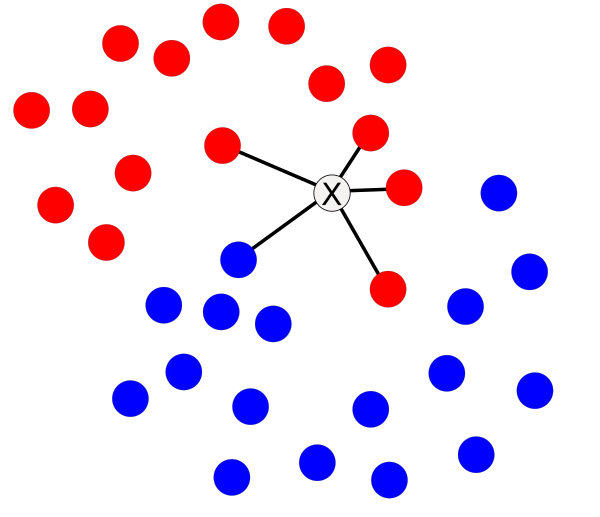
\includegraphics[width=50mm]{knn.png}%
    \caption{kNN classifier looks at k nearest neighbors, say 5, of instance X. 4 neighbors belong to the red class and 1 to the blue class. X will thus be classified as red with 80\% probability.}
\end{marginfigure}

Unlike most other algorithms, kNN does not construct a model but just stores the data. This kind of learning is called \textit{lazy learning}.

\begin{figure}[h]
    \centering
    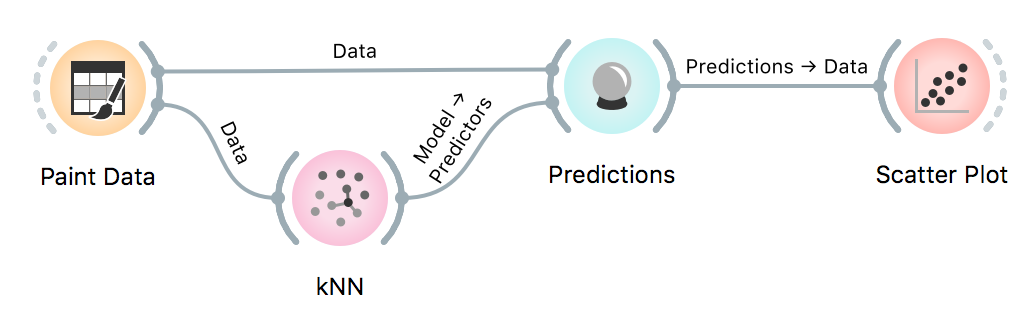
\includegraphics[width=\textwidth]{workflow.png}
    \caption{$\;$}
\end{figure}

The advantage of kNN algorithm is that it can successfully model the data, where classes are not linearly separably. It can also be re-trained quickly, because new data instances effect model only locally. However, the first training is can be slow for large data sets, as the model has to estimate k distances for data instance.

\begin{figure*}[h]
    \centering
    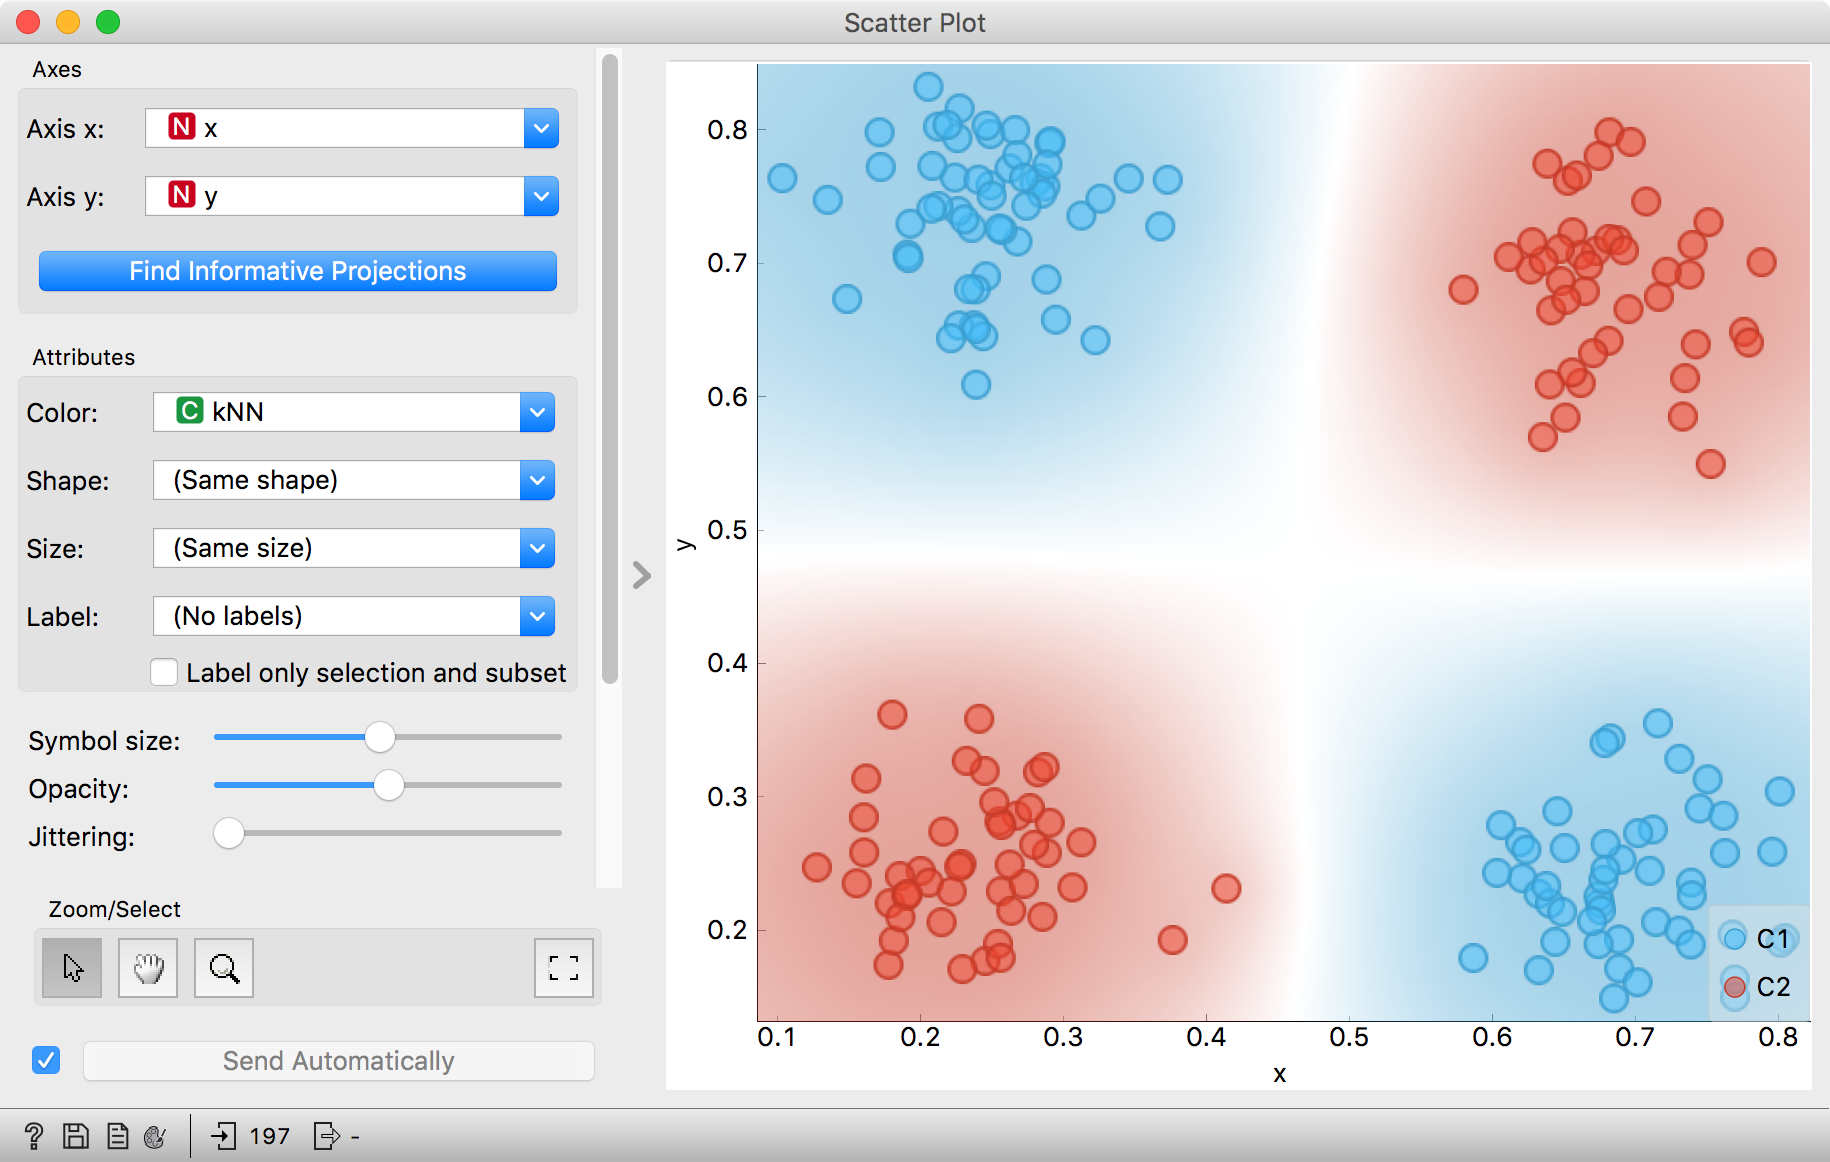
\includegraphics[scale=0.4]{knn-orange.png}
    \caption{$\;$}
\end{figure*}
